The goal of the VAns algorithm is to adaptively construct trainable ansatzes for generic problems encoded into a cost function, using parametrized quantum circuits. We will here consider general cost-functions of the form\footnote{More details can be found in Sec.~\ref{ssec:1_nisq_vqa}.}
\begin{equation}\label{eq:costbis}
    C(\kvec,\thv)=\sum_i^M f_i\left(\tr{O_i U(\kvec,\thv)\rho_i U^\dagger (\kvec,\thv)}\right),
\end{equation}
where $\{\rho_i\}_{i=1}^M$ are $n$-qubit states forming a training-set, and $U(\kvec,\thv)$ is our NISQ circuit parametrized by continuous parameters $\thv$ (\textit{e.g.}, rotation angles) and by discrete parameters $\kvec$ (\textit{e.g.}, gate placements); moreover $O_i$ are observables and $f_i$ are functions that encode the optimization task at hand.

We define $\CC_l$ as the architecture hyperspace of quantum circuits having $l$ gates in the layout. VAns takes as input:
\begin{itemize}
    \item A cost function $C(\kvec,\thv)$ to minimize.
    \item A dictionary $\DC$ of parametrized gates that compile to the identity. That is, for  $V(\gamv)\in\DC$ there exists a set of parameters $\gamv^*$ such that $V(\gamv^*)=\id$.
    \item An initial circuit configuration $U^{(0)}(\kvec,\thv)\in\CC_{l_0}$ of depth $l_0$ .
    \item Circuit \texttt{Insertion} rules which stochastically take an element $V(\gamv^*)\in\DC$ and randomly insert it in the circuit. The insertion is a map $\IC:\CC_l\rightarrow \CC_{l'}$ with $l'\geq l$.
    \item Circuit \texttt{Simplification} rules to eliminate unnecessary gates, redundant gates, or gates that do not have a large effect on the cost. The simplification is a map $\SC:\CC_l\rightarrow \CC_{l'}$ with $l'\leq l$.
    \item An optimization algorithm for the continuous parameters $\thv$, and an optimization algorithm for the discrete parameters $\kvec$.
\end{itemize}
Given these inputs, VAns outputs a circuit architecture and set of parameters that approximately minimize the cost function in Eq.~\ref{eq:costbis}.

In what follows we describe the overall structure of VAns (whose pseoudocode is provided later in this Section), and in the next sections we provide additional details for the \texttt{Insertion} and \texttt{Simplification} modules. We remark that the steps presented here are aimed at giving a general overview of the method and are intended to be used as building blocks for more advanced versions of VAns (which we discuss in Sec.~\ref{ssec:vans_discu}).

The first ingredient of VAns (besides the cost function, which is defined by the problem at hand) is a dictionary $\DC$ of parametrized gates that can compile to identity and which VAns employs to build the ansatz. A key aspect here is that $\DC$ can be composed of any set of gates, so that one can build a dictionary specifically tailored for a given application. In addition, it is usually convenient to have the unitaries in $\DC$ expressed in terms of gates native to the specific quantum hardware employed, as this avoids compilation depth overheads (\textit{e.g.} a larger number of gates would otherwise be required). In our numerics, we will consider a dictionary composed of one and two qubit identity block of gates that can resolve to the identity; the alphabet is given by single-qubit rotations and CNOT acting on any two qubits present in the circuit (see Sec.~\ref{ssec:insertion} for further details). As stressed in Sec.~\ref{ssec:1_nisq_vqa}, we will not consider issues arising from connectivity constraints.

Once the gate dictionary is set, the ansatz is initialized to a given configuration $U^{(0)}(\kvec,\thv)$. As discussed in Sec.~\ref{ssec:optimizer}, we then need to employ an optimizer to control the parameters $\thv$ of the initial ansatz until the convergence is reached. We recall that in Sec.~\ref{ssec:1_nisq_vans_bp} we discussed several strategies that define the ansatz structure. In particular, the two non-trivial ansatzes shown in Fig.~\ref{fig:FANSATZ} are employed in our numerical simulations as initialization strategies: \textit{(i)} the \textit{separable} product ansatz which generates no entanglement, and \textit{(ii)} the alternating \textit{Hardware Efficient Ansatz}
which entangles neighboring qubits; note that only shallow circuits (\textit{e.g.} a low number of HEA-layers) are considered for initialization purposes. While the choice of an appropriate initial ansatz can lead to faster convergence, VAns can in principle transform a simple initial ansatz into a more complex one as part of its architecture search.

From this point, VAns enters a nested optimization loop. In the outer loop, VAns explores the architecture hyperspace to optimize the ansatz's discrete parameters $\kvec$ that characterize the circuit structure. Then, in the inner loop, the ansatz structure is fixed and the continuous parameters $\thv$ are optimized.

At the start of the outer loop, VAns employs its \texttt{Insertion} rules to stochastically grow the circuit. The fact that these rules are stochastic guarantees that different runs of VAns explore distinct regions of the architecture hyperspace. As previously mentioned, the gates added to the circuit compile to the identity so that circuits that differ by gate insertions belong to an equivalence class of circuits leading to the same cost function value (we remark that this strategy has been also introduced in ~\cite{rattew2019domain}). As discussed below, the \texttt{Insertion} rules can be such that they depend on the current circuit they act upon. For instance, VAns can potentially add entangling gates to qubits that were not previously connected.

To prevent the circuit from constantly growing each time gates are inserted, VAns follows the \texttt{Insertion} step by a \texttt{Simplification} step. Here, the goal is to determine if the circuit can be compressec without significantly modifying the cost function value in a systematic way, as proposed in~\cite{maslov2008quantum}. This is a fundamental step of VAns as it allows the algorithm to explore and jump between different regions of the architecture hyperspace which might not be trivially connected. Moreover, unlike other variable-ansatz strategies that continuously grow the number of gates present in the circuit, or which randomly remove gates, the \texttt{Simplification} step allows VAns to find shorter ansatzes by deleting gates in an informed manner.

Taken together, \texttt{Insertion} and \texttt{Simplification} provide a set of discrete parameters $\kvec$. However, to determine if this new circuit structure can improve the cost function value it is necessary to enter the inner optimization loop and train the continuous parameters $\thv$. Here, we remark that a global optimization of all parameters shall be performed, since the landscape might contain a newer minima. In practice, when entering the continuous optimization, the parameters are initialized such that the circuit does not exactly compile to the same unitary than that of the previous step, but rather small perturbations are injected in order to help exiting potential local minima. When convergence in the optimization is reached, the final cost-function value is compared to the cost in the previous iteration. Updates that lead to equi-cost values or to smaller costs are accepted, while updates leading to higher cost functions are accepted with exponentially decaying probability in a manner similar to a Metropolis-Hastings step~\cite{hastings1970monte}. Here one accepts an update which increases the cost value with a probability given by $\exp{( -  \beta \frac{\Delta \mathcal{C}}{\mathcal{C}_0} )}$, with $\frac{\Delta \mathcal{C}}{\mathcal{C}_0}$ being increment in the cost function with respect to the initial value, and $\beta > 0$ a  \textit{temperature} factor.
The previous optimizations in inner and outer loops are repeated until a termination condition $f_\texttt{Term}$ is reached, \textit{e.g.} distance to a target cost function value (if a lower bound is available), maximum VAns iteration number, or an user-specified function that might depend on variables such as circuit structure and cost value reached.

In the following we will give more details about VAns specific modules.
\subsection{\texttt{Insertion} method}\label{ssec:insertion}
\begin{figure}[t]
\centering
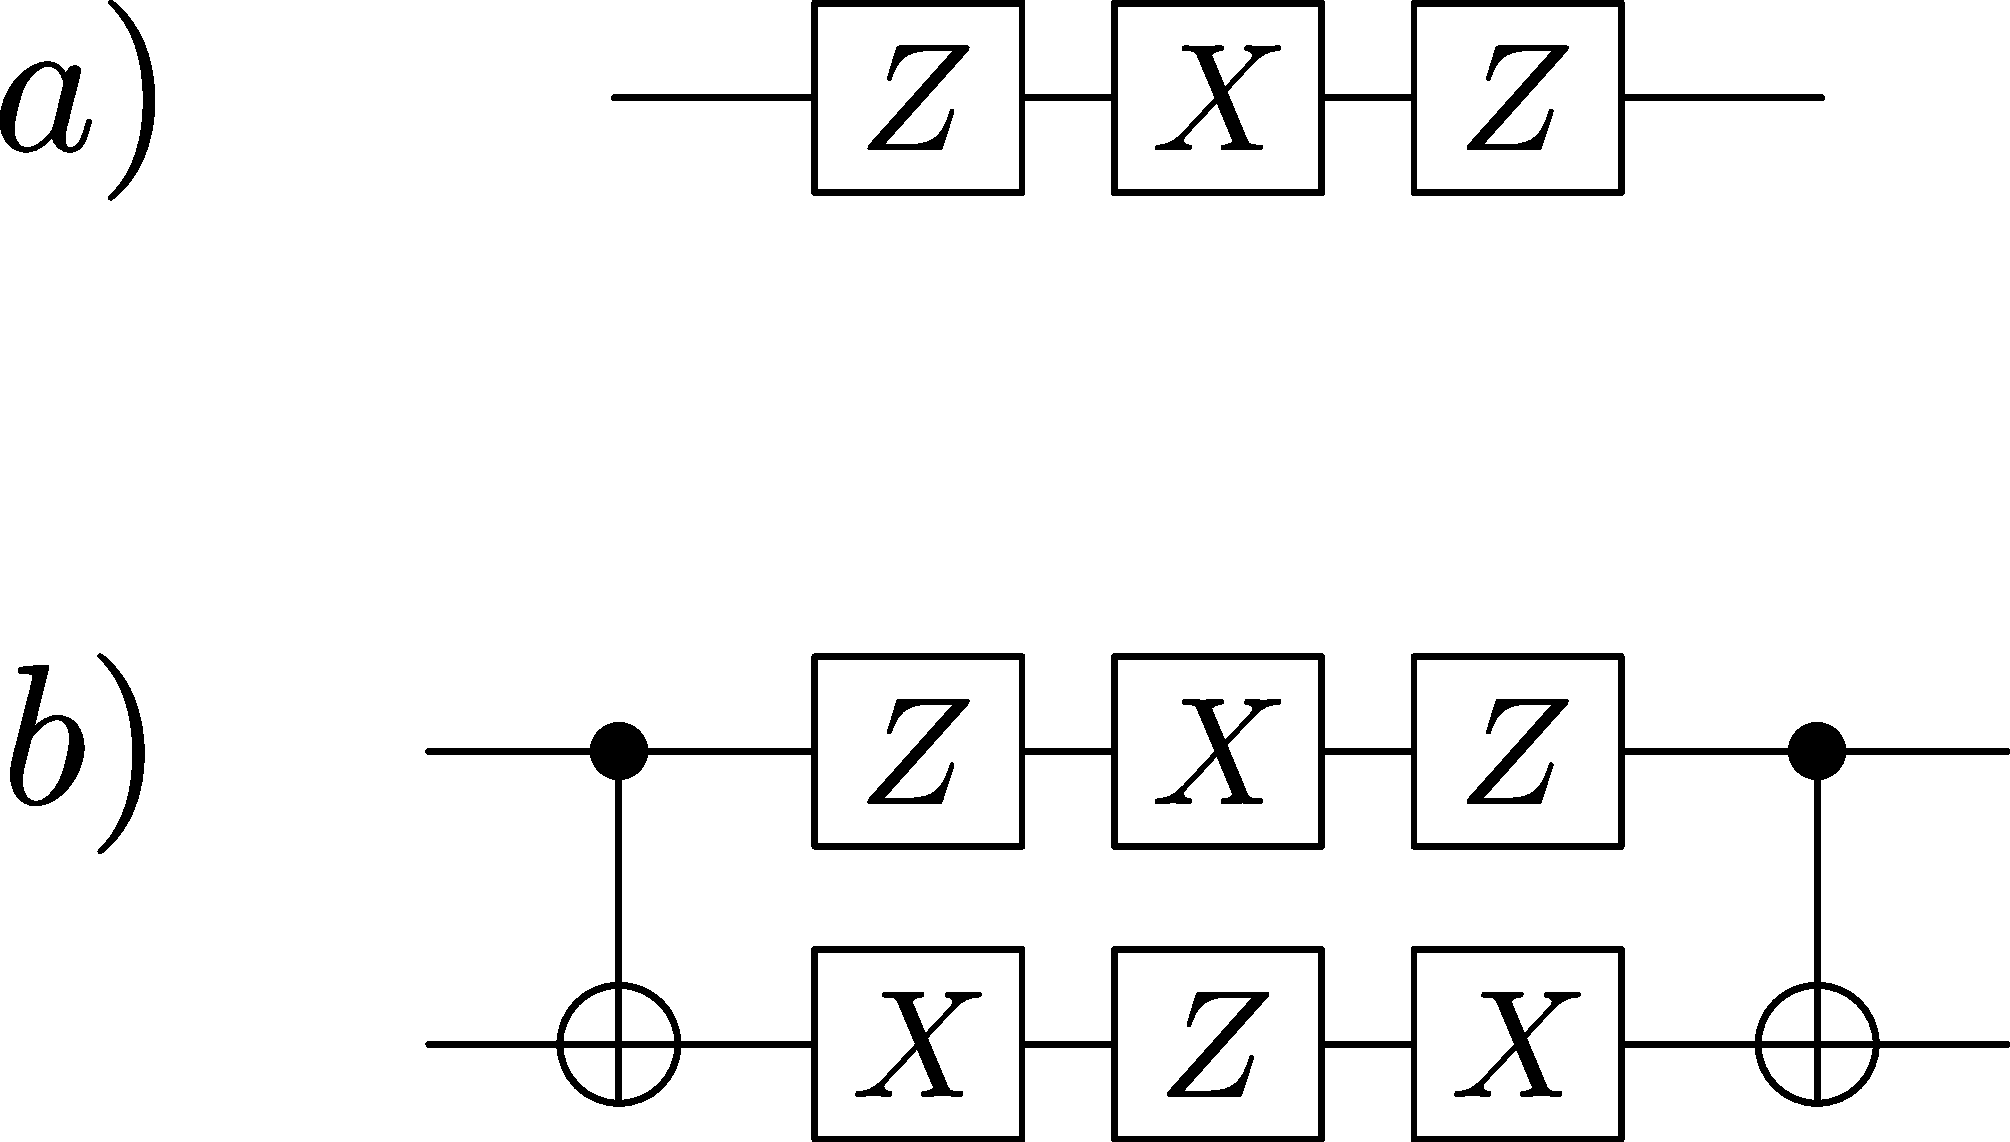
\includegraphics[width=.5\textwidth]{Figures/VANS/Fig3.pdf}
\caption{We show the two words from the dictionary $\DC$ used during the \texttt{Insertion} steps. Here we show two types of the parametrized gate sequences composed of CNOTs and rotations about the $z$ and $x$ axis. Specifically, one obtains the identity if the rotation angles are set to zero. Using the circuit in \textit{(a)}, one inserts a general unitary acting on a given qubit, while the circuit in \textit{(b)} correlates the two qubits it acts upon.}
\label{fig:blocks}
\end{figure}

The \texttt{Insertion} step stochastically grows the circuit by inserting a parametrized block of gates from the dictionary $\DC$ which compiles to the identity. In order to facilitate the exploration of a larger architecture-hyperspace region, in practice we allow some deviation from the identity by slightly modifying the continuous parameters so that the new gate deviates slightly from the identity. In Fig.~\ref{fig:blocks} we show examples of two parametrized quantum circuits that can compile to the identity.

There are many choices for how VAns determines which gates are chosen from $\DC$ at each iteration, and where they should be placed. When selecting gates, we have here taken a uniform sampling approach, where every sequence of gates in $\DC$ has an equal probability to be selected.

\subsection{\texttt{Simplification} method}
The \texttt{Simplification} steps in VAns are aimed at eliminating unnecessary gates, redundant gates, or gates that do not have a large effect on the cost. For this purpose, \texttt{Simplification} moves gates in the circuit using the commutation rules shown in Fig.~\ref{fig:simplification}(a) to group single qubits rotations and CNOTs together.
Once there are no further commutations possible, the circuit is scanned and a sequence of simplification rules are successively applied. For instance, assuming that the input state is initialized to $\ket{0}^{\otimes n}$, we can define the following set of simplification rules.
\begin{enumerate}
\item Scan the circuit for possible commutations: if possible place CNOTs at the left, and rotations at the right side.
\item CNOT gates acting at the beginning of the circuit are removed.
\item Rotations around the $z$-axis acting at the beginning of the circuit are removed.
\item Consecutive CNOT sharing the same control and target qubits are removed.
\item Two or more consecutive rotations around the same axis and acting on the same qubit are compiled into a single rotation (whose value is the sum of the previous values).
\item If three or more single-qubit rotations are sequentially acting on the same qubit, they are simplified into a general single-qubit rotation of the form $R_z(\theta_1) R_x(\theta_2) R_z(\theta_3)$ or $R_x(\theta_1) R_z(\theta_2) R_x(\theta_3)$ which has the same action as the previous product of rotations.
\item Gates whose presence in the circuit does not considerably reduce the cost are removed.
\end{enumerate}
Rules $(2)-(6)$ are schematically shown in Fig.~\ref{fig:simplification}(b). We remark that a crucial feature of these \texttt{Simplification} rules is that they can be performed using a classical computer that analyzes the circuit structure and hence do not lead to additional quantum-computation resources.

\begin{figure}[t!]
\centering
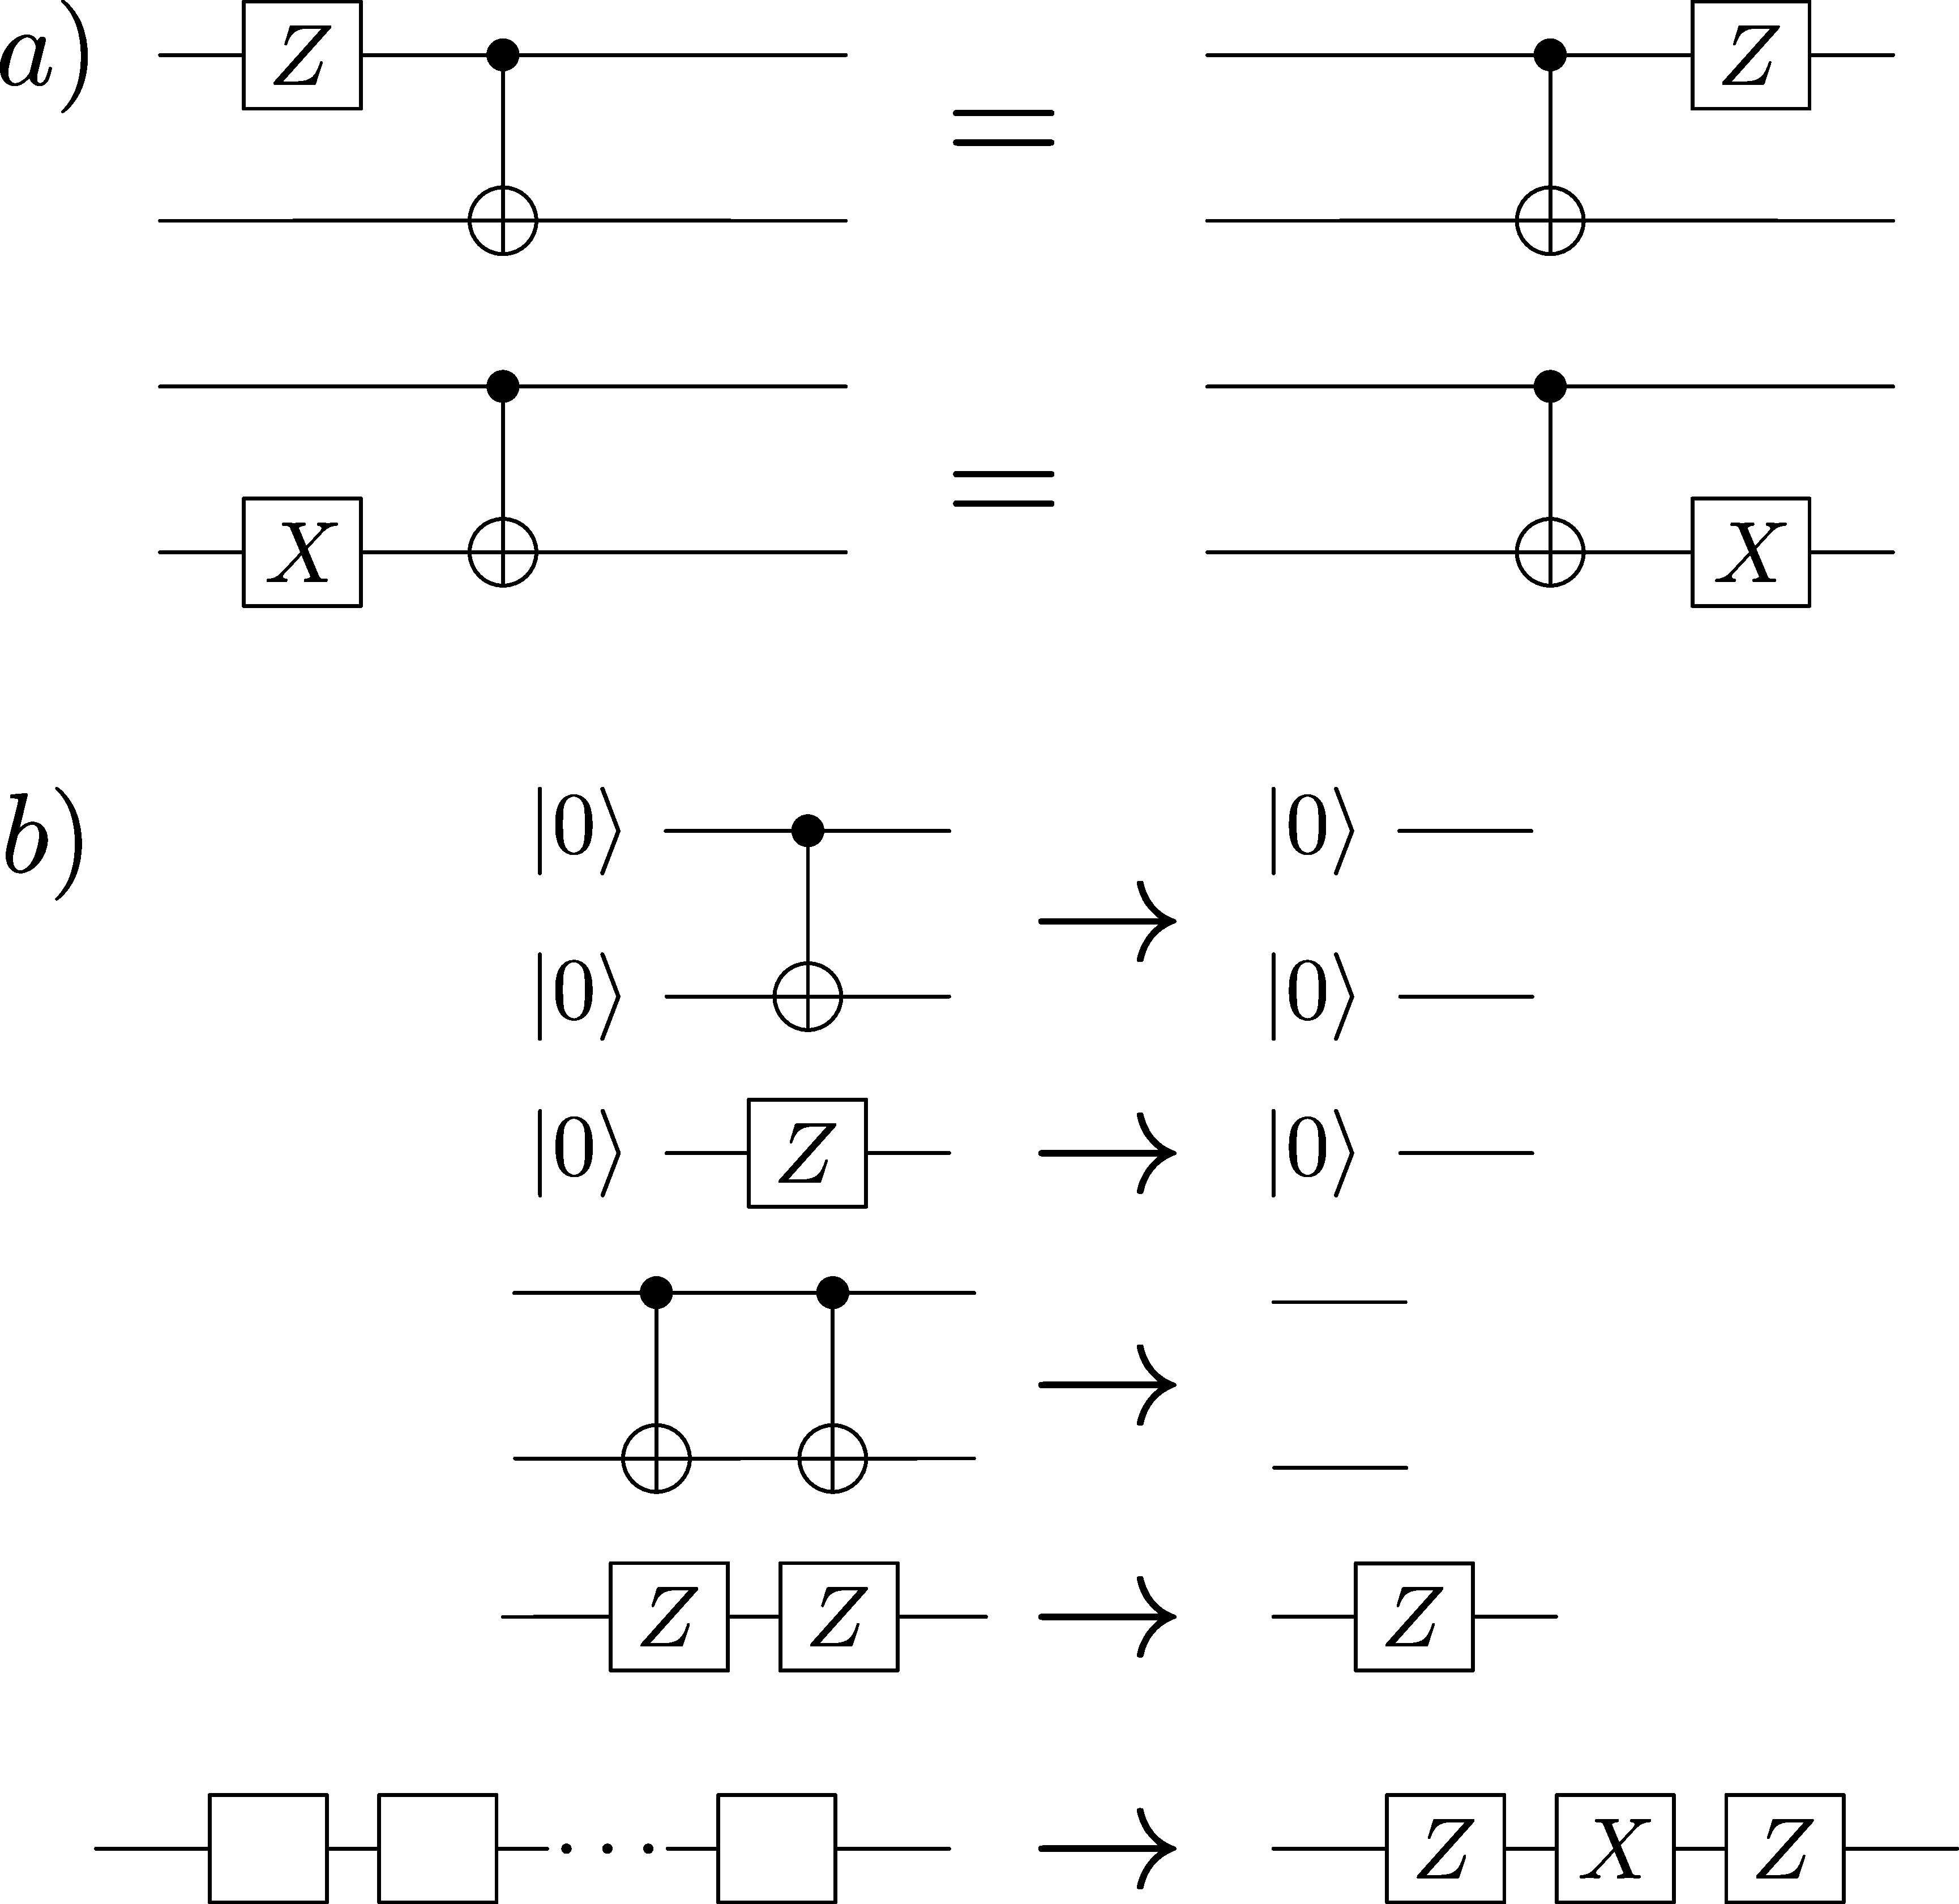
\includegraphics[width=.7\textwidth]{Figures/VANS/Fig4.pdf}
\caption{We depict the rules for the \texttt{Simplification} steps. \textit{(a)} Commutation rules used by VAns to move gates in the circuit. As shown, we can commute a CNOT with a rotation $Z$ ($X$) about the $z$ ($x$) axis acting on the control (target) qubit; when possible, CNOTs are moved to the left-side of the circuit, and rotations to the right one. \textit{(b)} Example of simplification rules used by VAns to reduce the circuit depth. Here we assume that the circuit is initialized to $\ket{0}^{\otimes n}$. }
\label{fig:simplification}
\end{figure}

As indicated by step $(6)$, the \texttt{Simplification} steps can also delete gates whose presence in the circuit does not considerably reduce the cost. Here, given a parametrized gate, one can remove it from the circuit and compute the ensuing cost function value. If the resulting cost is not increased by more than some threshold value, the gate under consideration is removed and the simplification rules $(1)-(5)$ are again implemented. Here, we can use information from the inner optimization loop to find candidate gates for removal. For instance, when employing a gradient descent optimizer, we may attempt to remove gates whose parameters lead to small gradients. Note that, unlike the simplification steps $(1)-(5)$ in Fig.~\ref{fig:simplification}\textit{(b)}, when using the deletion process in $(6)$ one needs to call a quantum computer to estimate the cost function, and hence these come at an additional quantum-resource overhead which scales linearly with the number of gates one is attempting to remove.

An interesting aspect of the \texttt{Simplification} method is that it allows VAns to obtain circuit structures that are not contained in the initial circuit $U^{(0)}(\kvec,\thv)$ or in the gate dictionary $\DC$, and hence to explore new regions of the architecture hyperspace. For instance, using the gate dictionary in Fig.~\ref{fig:blocks}, VAns can obtain a gate structure as the one shown in Fig.~\ref{fig:new}.

\begin{figure}[t!]
\centering
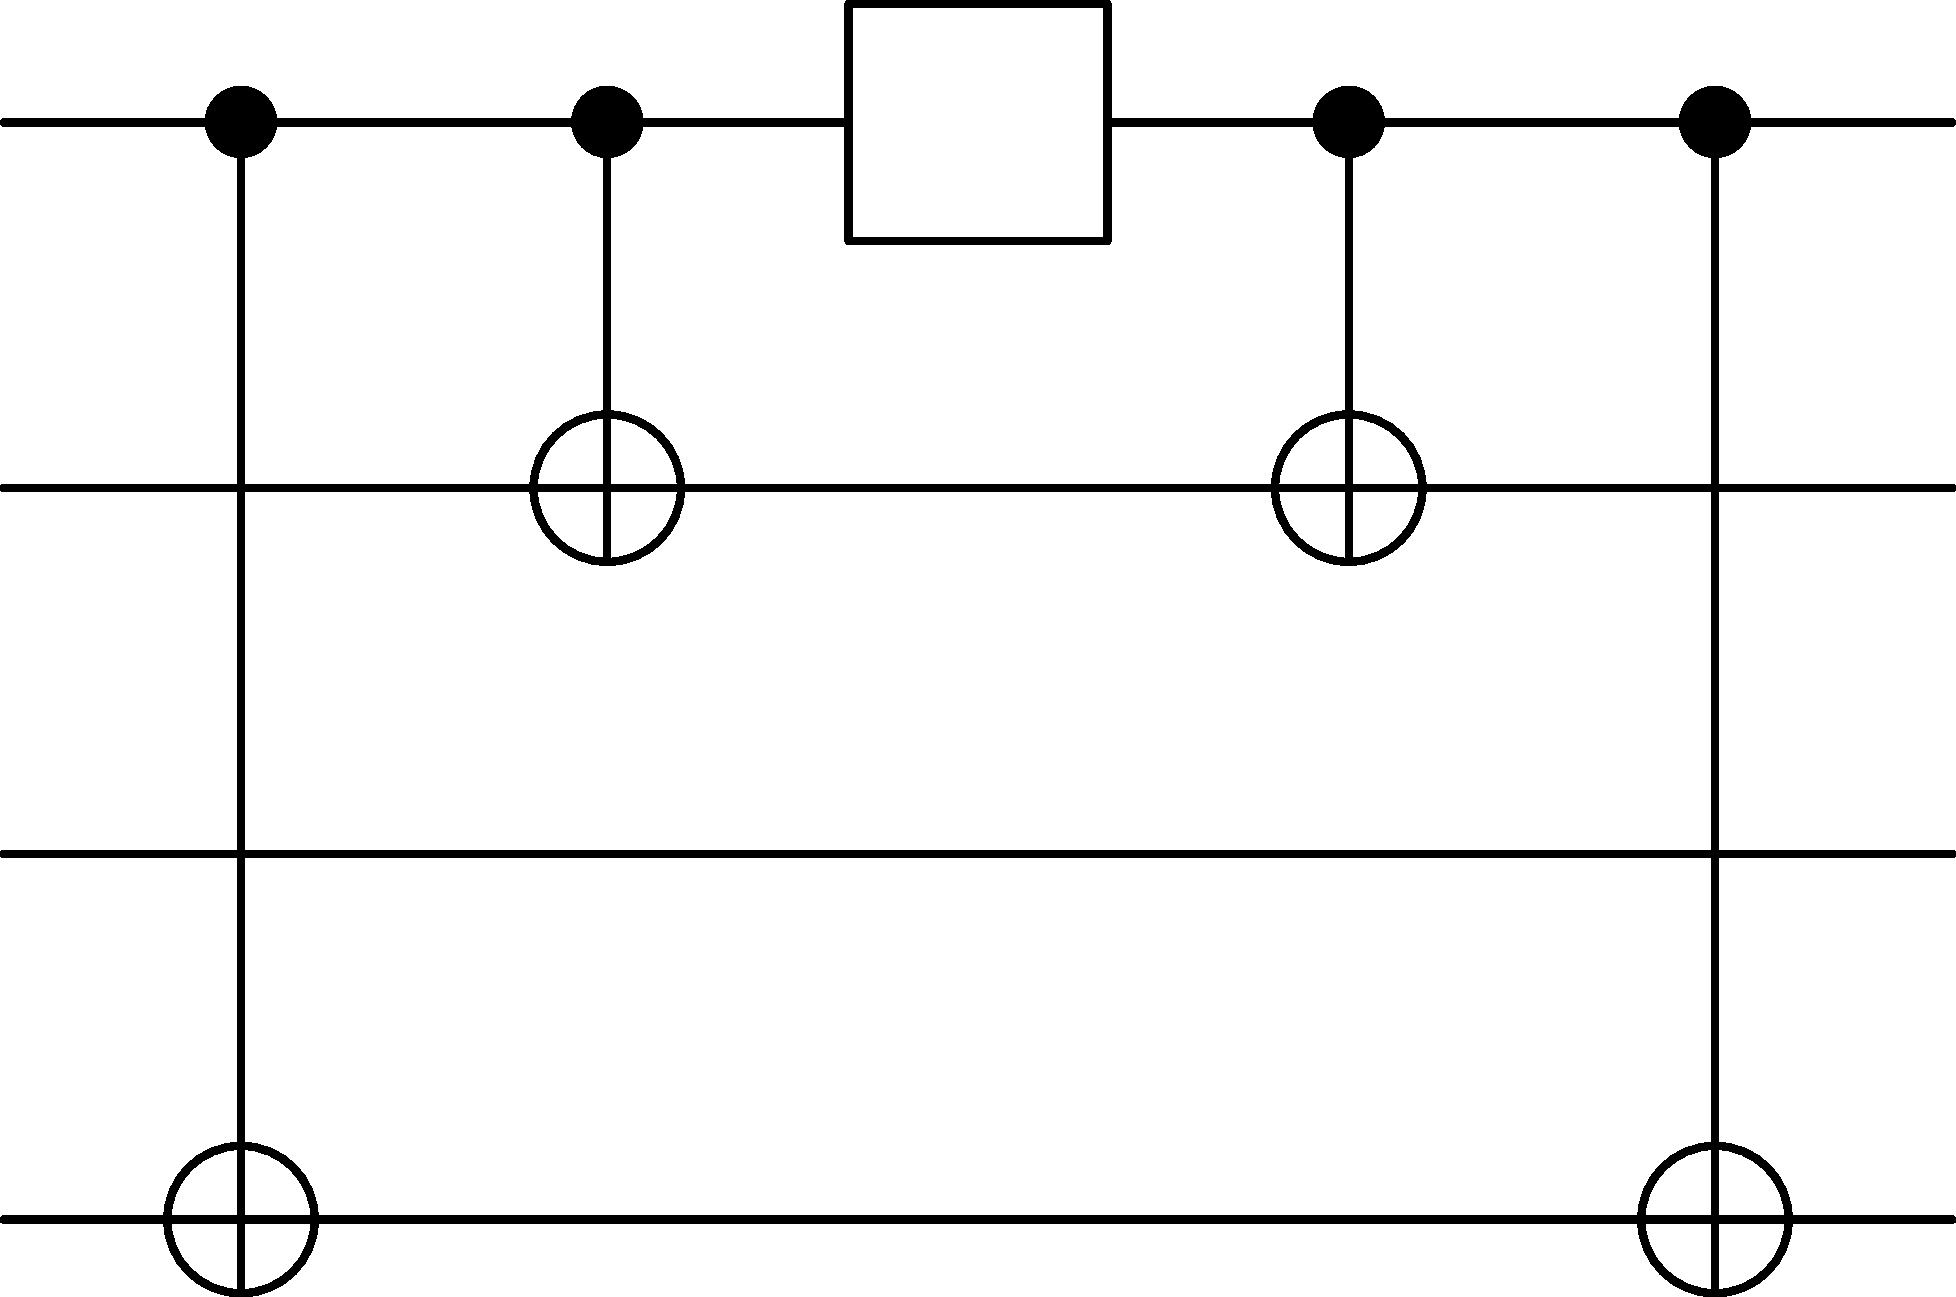
\includegraphics[width=.5\textwidth]{Figures/VANS/Fig5.pdf}
\caption{We show a non-trivial circuit structure that can be obtained by VAns using the \texttt{Insertion} and \texttt{Simplification} steps and the gate dictionary in Fig.~\ref{fig:blocks}. }
\label{fig:new}
\end{figure}
\afterpage{\clearpage}

\begin{algorithm}[h]\label{alg:algovans}
    \DontPrintSemicolon
    \KwIn{Cost function $C(\kvec,\thv)$; initial circuit $U^{(0)}(\kvec,\thv)$; dictionary of gates $\DC$; \texttt{Insertion} rules which take gates from $\DC$ and appends them to a circuit; \texttt{Simplification} rules; optimization algorithm \texttt{Opt}$_C$ for continuous parameters $\thv$; optimization algorithm \texttt{Opt}$_D$ for discrete parameters which accepts or rejects an ansatz update given changes in the cost function value; termination condition function $f_\texttt{Term}(n, C(\kvec,\thv),U(\kvec, \thv)), \; n\in \mathbb{N}$}
    \KwOut{Optimized ansatz $U^{(f)}$.}
    \kwInit{Randomly initialize the parameters $\thv$;
    initialize the ansatz $U^{(f)}\gets U^{(0)}(\kvec,\thv)$;
     $C^{(f)}\gets 0$;
    $\kvec^{(f)}\gets \kvec$;
    $\thv^{(f)}\gets \thv$;
    $\UC(\kvec,\thv)\gets \id$;
    $\texttt{Term} \leftarrow false$; $n \leftarrow 0$.
    }
    Optimize $\thv$ with \texttt{Opt}$_C$ and store result in $\thv^{(f)}$; $C^{(f)}\gets C(\kvec,\thv)$.\;
    \While{\texttt{Term} is false}{
    $n \leftarrow n + 1$\;
    $\texttt{Accept}\gets\textit{false}$\;
    \While{\texttt{Accept} is false}{
    Use \texttt{Insertion} in $U^{(f)}$ and store new sets of discrete parameters, continuous parameters and ansatz in $\thv$, $\kvec$, and  $\UC(\kvec,\thv)$, respectively.\;
    Use rules [1-6] of \texttt{Simplification} on $\UC(\kvec,\thv)$ and store new sets of discrete parameters, continuous parameters and ansatz in $\thv$, $\kvec$, and  $\UC(\kvec,\thv)$, respectively.\;
    Optimize continuous parameters in $\UC(\kvec,\thv)$ with \texttt{Opt}$_C$ and store result in $\thv$; $C^{(f)}\gets C(\kvec,\thv)$.\;
    Repeat step 7, with rules [1-7] of \texttt{Simplification}.\;
    Given $C(\kvec,\thv)$ and $C^{(f)}$, optimize discrete parameters in $\UC(\kvec,\thv)$ with \texttt{Opt}$_D$ and store result in \texttt{Accept}.\;
    }
    $\kvec^{(f)}\gets \kvec$.\;
    $\thv^{(f)}\gets \thv$.\;
    $U^{(f)}\gets \UC(\kvec,\thv)$.\;
    $C^{(f)}\gets C(\kvec,\thv)$.\;
    $\texttt{Term} \leftarrow f_{\texttt{Term}}(n,C^{(f)},U^{(f)})$
    }
    \caption{Pseudo-code for VAns}
 \end{algorithm}
\afterpage{\clearpage}
\newpage
\subsection{Scaling of VAns}

With the previous overview of the VAns method in mind, let us now discuss the computational complexity arising from using VAns versus that of using a standard fix architecture scheme. In the following discussion we will not include any computational cost or complexity of the continuous-parameter optimizer as we assume that the same tools could be used for fixed or variable ansatzes.

Firstly, we note that any additional computational cost comes due to circuit manipulations, meaning that we should study the scaling of the \texttt{Insertion} and \texttt{Simplification} methods. On the one hand, adding gates via \texttt{Insertion} is stochastic, and independent of the number of qubits or the current circuit depth, that is:  its complexity is always in $\OC(1)$. Then, removing gates via \texttt{Simplification} has a cost which increases with the number of gates in the circuit. If we have $M$ gates, then running the \texttt{Simplification} scheme has a cost $\OC(M)$. We note that such computational complexity is similar to that of using gradient-free versus gradient-based methods, as the computational cost of the latter also scale as $\OC(M)$. Notably, since the goal of VAns is to produce short-depth circuits, the algorithm itself tries to reduce its own computational cost during training.  As we sill see below in our numerical examples, VAns is always able to find short-depth circuits whose solutions are better than those arising from fixed structure ansatzes, meaning that the extra complexity of VAns can be justified in terms of its performance.

With an understanding of VAns mechanism, we will now turn to use it in a plethora of different scenarios.
